\documentclass[10pt,twocolumn,letterpaper]{article}

% CVPR style requires these before \usepackage{cvpr}
\def\confName{CVPR}
\def\confYear{2026}
\def\paperID{0000}

\usepackage[pagenumbers]{cvpr} % page numbers, no review ruler

\usepackage{graphicx}
\usepackage{amsmath}
\usepackage{amssymb}
\usepackage{booktabs}
\usepackage{times}
\usepackage{microtype}
\usepackage{caption}
\usepackage{subcaption}
\usepackage{tabularx}
\usepackage{multirow}
\usepackage{enumitem}
\usepackage{xcolor}
\usepackage{url}

\definecolor{cvprblue}{rgb}{0.21,0.49,0.74}
\usepackage[pagebackref,breaklinks,colorlinks,allcolors=cvprblue]{hyperref}
\usepackage[capitalize]{cleveref}
\crefname{section}{Sec.}{Secs.}
\crefname{table}{Table}{Tables}
\crefname{figure}{Fig.}{Figs.}
\frenchspacing

\begin{document}

\title{LSTM vs.\ Transformer Encoder for Text Classification:\\
A Controlled Comparison on AG News}

\author{Jihun Jang\\
University of Science and Technology (UST), ETRI School\\
Student ID 02521122\\
{\tt\small jhjang@vetec.co.kr}
}

\maketitle

\begin{abstract}
We present a controlled comparison of a recurrent encoder (LSTM) and a
self-attention encoder (Transformer) for AG News four-class topic
classification, with both models trained from scratch. We hold the data,
preprocessing, vocabulary, sequence length, and training budget fixed and
vary only the encoder, so that any difference in behaviour can be attributed
to the architecture rather than to confounding factors. Under identical
conditions the Transformer reaches $0.910$ test accuracy versus $0.833$ for
the LSTM at a comparable parameter count. Loss curves and a data-efficiency
ablation show that the gap stems from generalization: the LSTM overfits and
saturates at roughly $25\%$ of the data, whereas the Transformer scales
steadily. Removing positional encoding leaves accuracy unchanged, indicating
that the task is essentially bag-of-words and that the gap arises from
robustness, not word-order modelling. Token-importance analysis shows that
the Transformer distributes evidence across several topical tokens while the
LSTM can over-rely on a single token. The prior hypothesis that the
Transformer is more data-hungry is rejected.
\end{abstract}

\section{Introduction}
Recurrent networks such as the LSTM~\cite{hochreiter1997lstm} and
self-attention networks such as the Transformer~\cite{vaswani2017attention}
are the two most widely used sequence encoders. This project compares them on
AG News four-class news topic classification under identical conditions, with
both models trained from scratch. Our research question is: when the data,
preprocessing, vocabulary, sequence length, and training budget are all held
fixed, how do the two architectures differ in performance, convergence, data
efficiency, and error patterns? The goal is not to maximize accuracy itself
but to explain the cause of the difference. A controlled, head-to-head
comparison on the same task exposes the strengths and weaknesses of each
architecture.

\section{Dataset}
We use AG News from a single HuggingFace source, with four classes (0 World,
1 Sports, 2 Business, 3 Sci/Tech)~\cite{zhang2015character}. The test set is
reserved for final evaluation, and the validation set is formed by holding out
$10\%$ of the training set (seed 42). \Cref{tab:splits} summarizes the splits
and the class distribution; all four classes are balanced.

Preprocessing is identical for both models. After word-level tokenization
(lowercased), the vocabulary is built from the training set only (maximum size
$20{,}000$, minimum frequency 2, including padding and unknown tokens). Each
sentence is truncated or padded to a maximum length of 128, and padding
positions are ignored by masking. The training set contains $67{,}575$ unique
words; the $20{,}000$ most frequent cover $97.3\%$ of all token occurrences, so
only about $2.7\%$ of tokens map to the unknown token.

Label indexing is a common pitfall: the raw CSV uses labels $1$--$4$ whereas
the HuggingFace version uses $0$--$3$, which is directly compatible with the
$0$-based index required by the cross-entropy loss. Using a single source
avoids this confusion.

\begin{table}[t]
\centering\small
\begin{tabular}{lrr}
\toprule
Class & Train & Test \\
\midrule
World & $26{,}991$ & $1{,}900$ \\
Sports & $26{,}966$ & $1{,}900$ \\
Business & $27{,}100$ & $1{,}900$ \\
Sci/Tech & $26{,}943$ & $1{,}900$ \\
\midrule
\textbf{Total} & $\mathbf{108{,}000}$ & $\mathbf{7{,}600}$ \\
\bottomrule
\end{tabular}
\caption{Per-class counts. Validation is $12{,}000$ ($10\%$ held out from
Train, seed 42). All classes are balanced.}
\label{tab:splits}
\end{table}

\section{Models}
Both models share the same skeleton: an embedding layer (dimension 128), an
encoder, masked mean pooling, and a linear output layer (4 classes), trained
with the cross-entropy loss. Only the encoder in the middle differs. This
control is the core of the comparison and lets us attribute performance
differences to the architecture. \Cref{tab:models} lists the configurations.
Because the embedding (about $2.56$M parameters) dominates both models, the
total parameter counts differ by only about $14\%$ and are therefore
comparable.

Implementation details: the padding token is fixed at index 0 and registered
as the embedding padding index, so its vector is never trained. Pooling and
self-attention ignore padding positions via masking. Both models use the same
masked mean pooling, so that the pooling method is not a confounding factor.

\begin{table}[t]
\centering\small
\setlength{\tabcolsep}{4pt}
\begin{tabularx}{\columnwidth}{lXX}
\toprule
 & LSTM & Transformer \\
\midrule
Embed.\ dim & 128 & 128 \\
Encoder & bidirectional LSTM, 2 layers, hidden 128 & 2 layers, 4 heads, FFN 256, sinusoidal PE \\
Output dim & 256 (bi) & 128 \\
Pool / Loss & masked mean / CE & masked mean / CE \\
Params & $3{,}220{,}484$ & $2{,}825{,}476$ \\
\bottomrule
\end{tabularx}
\caption{Model configurations. Only the encoder differs; the embedding,
pooling, and head are identical.}
\label{tab:models}
\end{table}

\section{Experiments}
The training setup is the Adam optimizer~\cite{kingma2015adam} with learning
rate $0.001$, batch size 64, up to 8 epochs, dropout $0.1$, and seed 42. Model
selection uses the best checkpoint by validation performance only, and the
test set is evaluated exactly once. Training runs on Apple MPS.

The main comparison trains both models with the setup above. The ablation
measures data efficiency by reducing the training set to $5\%$, $25\%$, $50\%$,
and $100\%$. The vocabulary is built once on the full training set and reused
unchanged at every fraction; subsets are stratified by class with a fixed
seed; the validation and test sets are always used in full. The evaluation
metrics are accuracy, macro F1-score, training/validation loss curves, and
confusion matrices. For a fair comparison the split, tokenizer, vocabulary,
maximum length, pooling, optimizer, learning rate, batch size, number of
epochs, and seed are all identical across the two models; the only variable is
the encoder.

\section{Results}
\Cref{tab:main} shows that the Transformer leads by about $7.7$ percentage
points at a comparable parameter count.

\begin{table}[t]
\centering\small
\begin{tabular}{lcc}
\toprule
Model & Test accuracy & Test macro F1 \\
\midrule
LSTM & $0.833$ & $0.835$ \\
Transformer & $\mathbf{0.910}$ & $\mathbf{0.909}$ \\
\bottomrule
\end{tabular}
\caption{Main results under identical conditions.}
\label{tab:main}
\end{table}

\begin{figure*}[t]
\centering
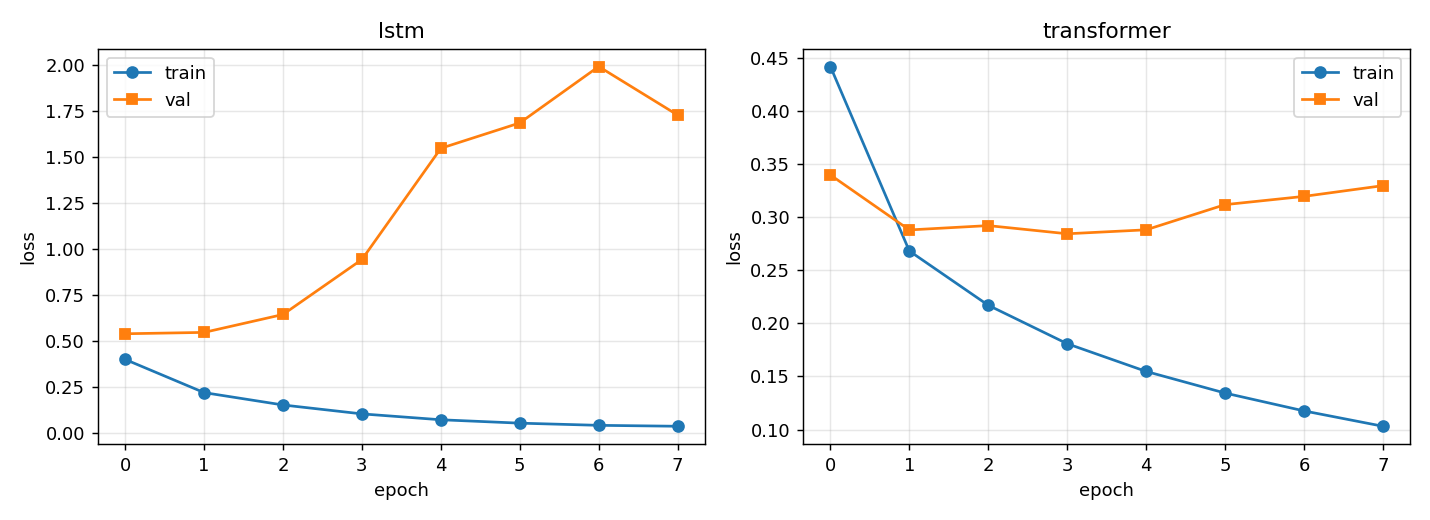
\includegraphics[width=0.92\textwidth]{fig_loss_curves.png}
\caption{Training and validation loss curves (left: LSTM, right:
Transformer). The LSTM overfits (validation loss rises to about $2.0$), while
the Transformer keeps validation loss flat.}
\label{fig:loss}
\end{figure*}

The learning curves are direct evidence of the gap (\cref{fig:loss}). For the
LSTM, the training loss falls to $0.035$ while the validation loss rises from
$0.54$ to about $2.0$, a textbook case of overfitting. The Transformer keeps
its validation loss flat (about $0.28$ to $0.33$) with almost no overfitting
and converges quickly, already reaching $88\%$ accuracy after the first epoch.
Because the best checkpoint by validation is saved before overfitting (epoch
2), the LSTM still secures its final score.

The confusion patterns (\cref{fig:cm}) are as follows. In the LSTM, Business is
mostly misclassified as Sci/Tech (258 cases) and Sci/Tech mostly as Business
(154 cases), so the mutual confusion between these two classes is largest.
World and Sports have similar error distributions, both misclassified mainly as
Business and Sci/Tech; as a result the LSTM makes substantial errors in every
class, spread across the board. In the Transformer, errors concentrate almost
entirely on the Business/Sci-Tech boundary (Business as Sci/Tech 147 cases,
Sci/Tech as Business 138 cases), while Sports is near-perfect (38 errors) and
World is clean.

\begin{figure*}[t]
\centering
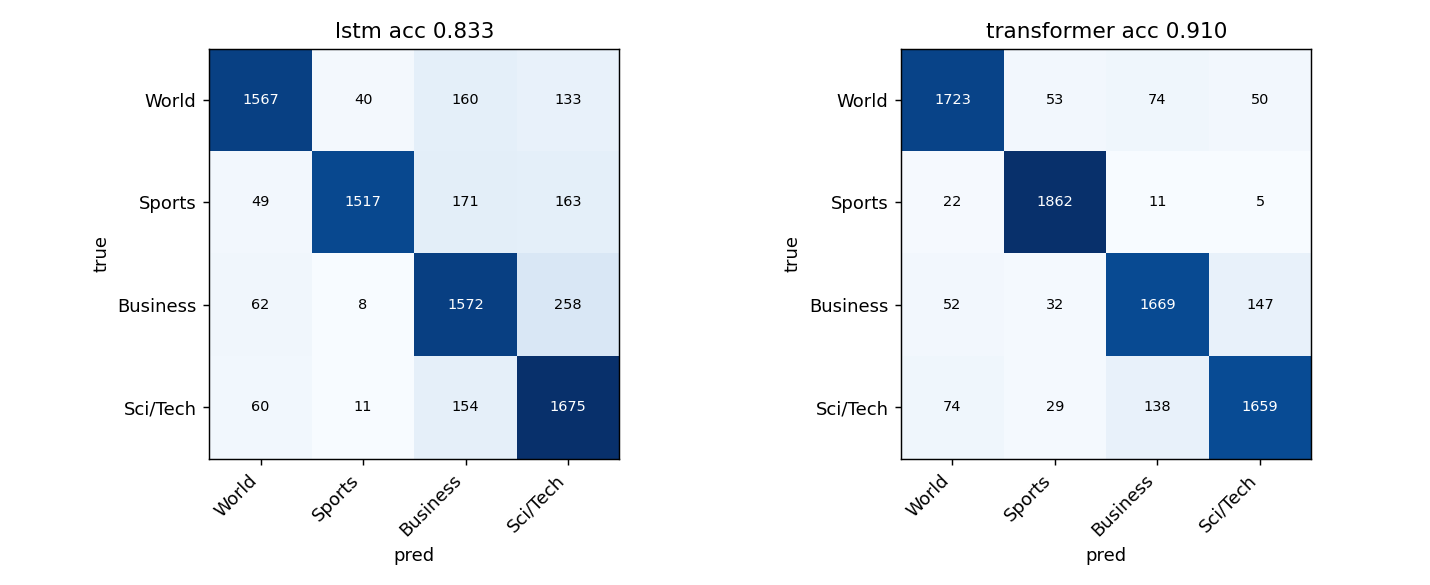
\includegraphics[width=0.92\textwidth]{fig_confusion.png}
\caption{Confusion matrices (row: true label, column: predicted label). Both
models confuse Business and Sci/Tech most; the LSTM additionally errs across
all classes.}
\label{fig:cm}
\end{figure*}

The shared trait is that both models confuse Business and Sci/Tech the most,
because the two classes share business, technology, and market vocabulary; the
cause is semantic overlap, not sequence length. Per class, the Transformer is
especially strong on Sports and World and weak only on Business and Sci/Tech.
The LSTM is not as strong as the Transformer even on Sports and World, making
non-trivial errors even where the vocabulary is distinctive.

The data-efficiency ablation (\cref{fig:abl}, \cref{tab:abl}) is revealing. The
Transformer improves monotonically as data grows. The LSTM peaks at $25\%$
($0.846$) and then plateaus; adding more data does not help because of
overfitting. In other words, the LSTM saturates at about the $25\%$ point and
cannot exploit additional data, while the Transformer scales steadily with
data. Because the Transformer leads at every fraction, the prior hypothesis
that the Transformer requires more training data (i.e., is less data-efficient)
is rejected for this task. AG News is a relatively easy task, so the
Transformer generalizes well even at the $5{,}400$-example scale.

\begin{table}[t]
\centering\small
\begin{tabular}{lccc}
\toprule
Training data & LSTM & Transformer & Gap \\
\midrule
$5\%$ ($5{,}399$) & $0.727$ & $0.798$ & $+0.071$ \\
$25\%$ ($26{,}998$) & $0.846$ & $0.875$ & $+0.029$ \\
$50\%$ ($53{,}999$) & $0.833$ & $0.897$ & $+0.064$ \\
$100\%$ ($108{,}000$) & $0.833$ & $\mathbf{0.910}$ & $+0.077$ \\
\bottomrule
\end{tabular}
\caption{Data-efficiency ablation: test accuracy vs.\ training-set size.}
\label{tab:abl}
\end{table}

\begin{figure}[t]
\centering
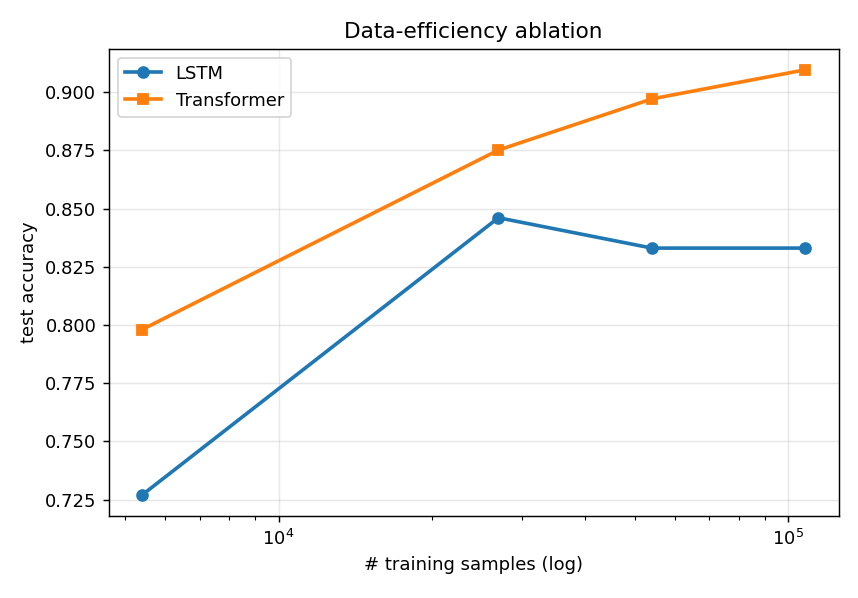
\includegraphics[width=\columnwidth]{fig_ablation.png}
\caption{Data-efficiency ablation. Test accuracy versus training-set size. The
LSTM saturates at $25\%$; the Transformer keeps improving.}
\label{fig:abl}
\end{figure}

Training efficiency also differed. On Apple MPS, the per-epoch training time
was about $47$\,s for the Transformer versus about $56$\,s for the LSTM, because
self-attention parallelizes computation across positions whereas the LSTM
processes tokens sequentially. The Transformer thus led in both accuracy and
training speed.

Overall, the performance gap stems from generalization and overfitting rather
than from sequence-order modelling (which, as the next section shows, this task
barely uses).

\section{Failure Analysis}
By category, both models are wrong on 428 cases, the LSTM alone on 841, and the
Transformer alone on 259. The LSTM's solo errors are about $3.2\times$ more
frequent, which supports the accuracy gap. Of the cases both models miss,
$61\%$ have a true label of Business or Sci/Tech; these are ambiguous boundary
cases that reflect class overlap in the task rather than a model defect
(\cref{tab:fail}).

Confidence patterns also differ. Shared errors often come with high confidence:
on the Intel example both models were wrong with confidence above $0.98$, an
overconfident boundary error. LSTM-only errors, by contrast, often carry low
confidence ($0.50$--$0.59$), indicating misclassification under the model's own
uncertainty and suggesting a lack of robustness. In short, the two models fail
in different ways.

\begin{table*}[t]
\centering\footnotesize
\begin{tabularx}{\textwidth}{XlllX}
\toprule
Article (summary) & True & LSTM & Transf. & Likely cause \\
\midrule
Some People Not Eligible to Get in on Google IPO & Sci/Tech & Business & Business & Corporate IPO blurs the finance/technology boundary \\
Intel to delay product aimed for high-definition TVs & Business & Sci/Tech & Sci/Tech & Tech vocabulary but a business-impact label; both wrong with high confidence \\
Teenage T.\ rex's monster growth & Sci/Tech & Business & Sci/Tech & Clearly science; only the LSTM errs, with low confidence \\
IBM to hire even more new workers & Sci/Tech & Business & Sci/Tech & Hiring story; boundary is ambiguous; only the Transformer is correct \\
Prediction Unit Helps Forecast Wildfires & Sci/Tech & Sci/Tech & Sports & A rare Transformer error \\
\bottomrule
\end{tabularx}
\caption{Representative misclassifications and their likely causes.}
\label{tab:fail}
\end{table*}

\section{Extension: Transformer Mechanism Analysis}
We carried out all three planned mechanism analyses; only the
positional-encoding experiment requires extra training, while the others reuse
the trained models.

First, a positional-encoding on/off experiment. Retraining the Transformer
without positional encoding leaves test accuracy essentially unchanged ($0.910$
to $0.911$, a difference of $-0.001$). Without positional encoding,
self-attention is a set encoder with no order information~\cite{vaswani2017attention};
identical accuracy therefore indicates that AG News is bag-of-words in nature,
where token occurrence matters more than word order, and that the
order-injecting component is unnecessary for this task.

Second and third, token-importance analyses via gradient saliency and attention
weights. \Cref{fig:mech} compares which tokens each model relies on for the same
Sports article. The LSTM assigns the largest importance to ``giddy,'' a word
unrelated to the topic, and misclassifies the article as Sci/Tech. The
Transformer spreads importance across topical tokens such as ``phelps,''
``seconds,'' ``medley,'' and ``400,'' with gradient saliency and attention
weights showing the same trend, and classifies the article correctly as Sports.
In other words, the Transformer distributes its evidence across several topical
tokens, whereas the LSTM can over-rely on a single token; this reveals a
token-level cause of the accuracy gap. We note that gradient saliency and
attention weights do not coincide exactly, so attention weights should not be
equated directly with explanation.

\begin{figure*}[t]
\centering
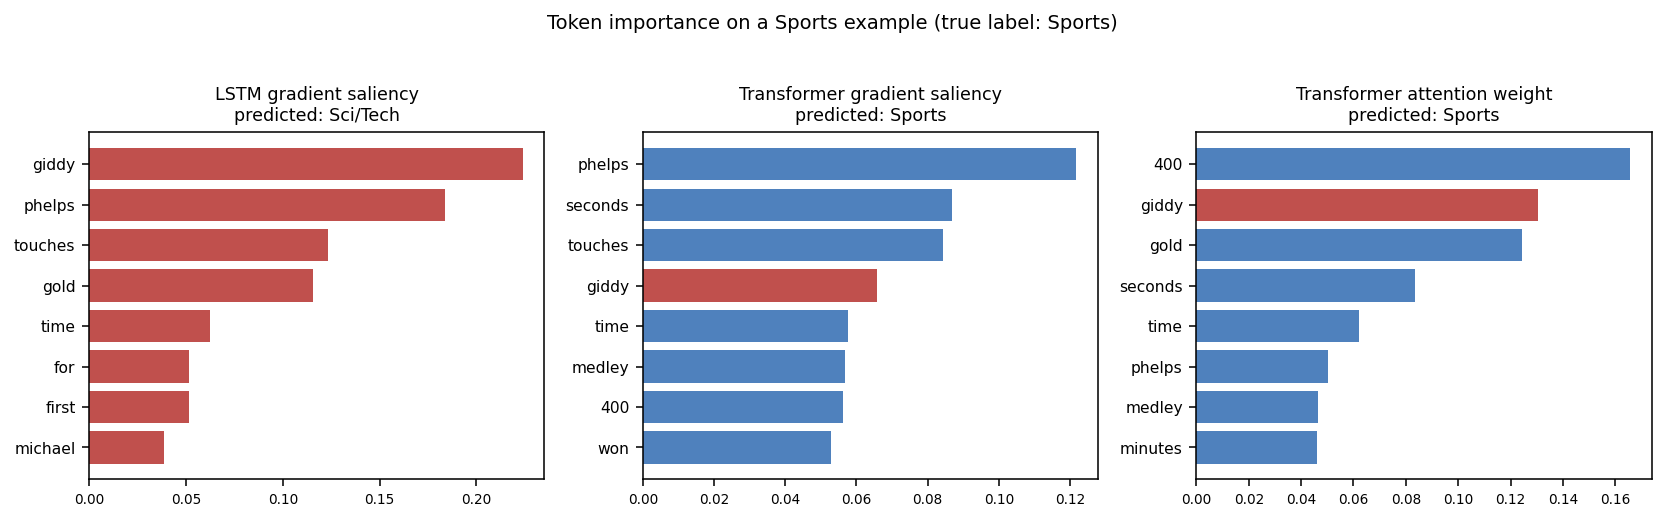
\includegraphics[width=\textwidth]{fig_mechanism.png}
\caption{Token importance on a Sports example (true label: Sports). Left: LSTM
gradient saliency (misclassified as Sci/Tech). Centre and right: Transformer
gradient saliency and attention weight (both correct).}
\label{fig:mech}
\end{figure*}

\section{Conclusion}
\begin{itemize}[leftmargin=1.2em,itemsep=2pt,topsep=2pt]
\item Under identical conditions the Transformer is clearly superior to the
LSTM ($0.910$ vs.\ $0.833$ test accuracy).
\item The cause is a difference in generalization. The LSTM overfits severely
and saturates at roughly $25\%$ of the data, failing to exploit additional
data, whereas the Transformer scales steadily.
\item The task is essentially bag-of-words: removing positional encoding does
not affect accuracy, so the gap arises from robustness and generalization
rather than word-order modelling.
\item The prior hypothesis that the Transformer needs more training data is
rejected; the Transformer leads at every data fraction.
\item \textbf{Limitations and future work.} Results are based on a single seed
and should be re-confirmed across seeds. Stronger regularization (e.g.,
dropout) for the LSTM may narrow the gap. The effect of positional encoding
should be re-examined on order-sensitive tasks (sentiment analysis, natural
language inference), and a word-order-shuffling ablation could compare the two
architectures' order sensitivity more directly.
\end{itemize}

{\small
\bibliographystyle{ieeenat_fullname}
\bibliography{references}
}

\end{document}
